\documentclass{article}
\usepackage[T1]{fontenc}
\usepackage{lmodern}
\usepackage{graphicx}
\usepackage{amsmath,amssymb}
\usepackage[a4paper,margin=2cm]{geometry}
\usepackage[absolute,overlay]{textpos}
\setlength{\TPHorizModule}{1mm}
\setlength{\TPVertModule}{1mm}
\usepackage[indonesian]{babel}
\usepackage{hyperref}
\setlength{\emergencystretch}{2em}
% unit: Halaman 108

\begin{document}

% === Halaman 108 (python/native) ===

108

E. Enigma Cipher

• Enigma adalah mesin enkripsi elektromekanik 

untuk melakukan enkripsi dan dekripsi.  

• Ditemukan dan dipatenkan oleh insinyur Jerman, 

Arthur Scherbius, untuk tujuan komersil, 

diplomatik, dan militer

• Menjadi terkenal karena digunakan oleh tantara 

Nazi Jerman selama Perang Dunia II untuk 

mengenkripsi/dekripsi pesan-pesan militer. 

• Enigma berasal dari bahasa latin, enigmae, yang 

artinya teka-teki.

% deskripsi: gambar native xref 384
\noindent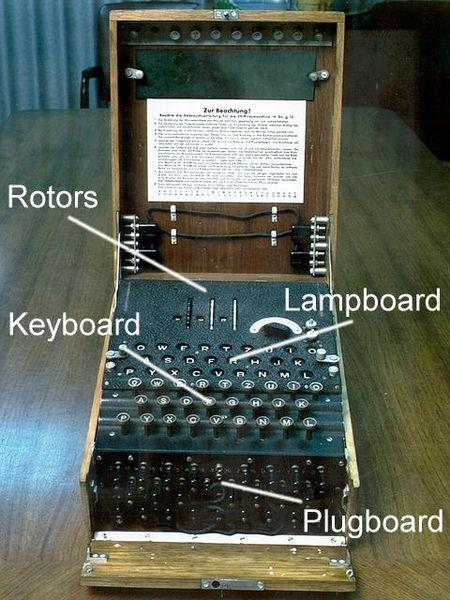
\includegraphics[width=0.85\textwidth]{../../images/python/page_108_img_01.jpeg}

\end{document}
